%----------------------------------------------------------------------------------------
%	PACKAGES AND OTHER DOCUMENT CONFIGURATIONS
%----------------------------------------------------------------------------------------

\documentclass{article}

\usepackage{fancyhdr} % Required for custom headers
\usepackage{lastpage} % Required to determine the last page for the footer
\usepackage{extramarks} % Required for headers and footers
\usepackage{graphicx} % Required to insert images
\usepackage{amsmath, amssymb} % Required for Maths
\usepackage{mathtools} % Required for Maths
\usepackage{enumerate}
\usepackage{mathtools}
\usepackage{textcomp}
\usepackage{gensymb}
\usepackage{siunitx}
\usepackage{spverbatim}
\usepackage{empheq}
\usepackage{ulem}
\usepackage{amssymb}
\usepackage{listings} % Required for insertion of code
\usepackage[usenames,dvipsnames]{xcolor} % Required for custom colors

% Margins
\topmargin=-0.45in
\evensidemargin=0in
\oddsidemargin=0in
\textwidth=6.5in
\textheight=9.0in
\headsep=0.25in 

\linespread{1.1} % Line spacing

% Set up the header and footer
\pagestyle{fancy}
\lhead{\hmwkAuthorName} % Top left header
\chead{\hmwkClass\ (\hmwkClassInstructor\ \hmwkClassTime): \hmwkTitle} % Top center header
\rhead{\firstxmark} % Top right header
\lfoot{\lastxmark} % Bottom left footer
\cfoot{} % Bottom center footer
\rfoot{Page\ \thepage\ of\ \pageref{LastPage}} % Bottom right footer
\renewcommand\headrulewidth{0.4pt} % Size of the header rule
\renewcommand\footrulewidth{0.4pt} % Size of the footer rule

\setlength\parindent{0pt} % Removes all indentation from paragraphs


%----------------------------------------------------------------------------------------
%	CODE INCLUSION CONFIGURATION
%----------------------------------------------------------------------------------------

\definecolor{MyDarkGreen}{rgb}{0.0,0.4,0.0} % This is the color used for comments
\lstloadlanguages{Matlab} % Load Perl syntax for listings, for a list of other languages supported see: ftp://ftp.tex.ac.uk/tex-archive/macros/latex/contrib/listings/listings.pdf
\lstset{language=Matlab, % Use Perl in this example
        frame=single, % Single frame around code
        breakatwhitespace=true,
        breaklines = true,
        basicstyle=\small\ttfamily, % Use small true type font
        keywordstyle=[1]\color{Blue}\bf, % Perl functions bold and blue
        keywordstyle=[2]\color{Purple}, % Perl function arguments purple
        keywordstyle=[3]\color{Blue}\underbar, % Custom functions underlined and blue
        identifierstyle=, % Nothing special about identifiers                                         
        commentstyle=\usefont{T1}{pcr}{m}{sl}\color{MyDarkGreen}\small, % Comments small dark green courier font
        stringstyle=\color{Purple}, % Strings are purple
        showstringspaces=false, % Don't put marks in string spaces
        tabsize=5, % 5 spaces per tab
        %
        % Put standard Perl functions not included in the default language here
        morekeywords={rand},
        %
        % Put Perl function parameters here
        morekeywords=[2]{on, off, interp},
        %
        % Put user defined functions here
        morekeywords=[3]{test},
       	%
        morecomment=[l][\color{Blue}]{...}, % Line continuation (...) like blue comment
        numbers=left, % Line numbers on left
        firstnumber=1, % Line numbers start with line 1
        numberstyle=\tiny\color{Blue}, % Line numbers are blue and small
        stepnumber=1 % Line numbers go in steps of 1
        }

% Creates a new command to include a script, the first parameter is the filename of the script (without .pl), the second parameter is the caption
\newcommand{\script}[2]{
\begin{itemize}
\item[]\lstinputlisting[caption=#2,label=#1]{#1.m}
\end{itemize}
}

%----------------------------------------------------------------------------------------
%	DOCUMENT STRUCTURE COMMANDS
%	Skip this unless you know what you're doing
%----------------------------------------------------------------------------------------

% Header and footer for when a page split occurs within a problem environment
\newcommand{\enterProblemHeader}[1]{
\nobreak\extramarks{#1}{#1 continued on next page\ldots}\nobreak
\nobreak\extramarks{#1 (continued)}{#1 continued on next page\ldots}\nobreak
}

% Header and footer for when a page split occurs between problem environments
\newcommand{\exitProblemHeader}[1]{
\nobreak\extramarks{#1 (continued)}{#1 continued on next page\ldots}\nobreak
\nobreak\extramarks{#1}{}\nobreak
}

\setcounter{secnumdepth}{0} % Removes default section numbers
\newcounter{homeworkProblemCounter} % Creates a counter to keep track of the number of problems

\newcommand{\homeworkProblemName}{}
\newenvironment{homeworkProblem}[1][Problem \arabic{homeworkProblemCounter}]{ % Makes a new environment called homeworkProblem which takes 1 argument (custom name) but the default is "Problem #"
\stepcounter{homeworkProblemCounter} % Increase counter for number of problems
\renewcommand{\homeworkProblemName}{#1} % Assign \homeworkProblemName the name of the problem
\section{\homeworkProblemName} % Make a section in the document with the custom problem count
\enterProblemHeader{\homeworkProblemName} % Header and footer within the environment
}{
\exitProblemHeader{\homeworkProblemName} % Header and footer after the environment
}

\newcommand{\problemAnswer}[1]{ % Defines the problem answer command with the content as the only argument
\noindent\framebox[\columnwidth][c]{\begin{minipage}{0.98\columnwidth}#1\end{minipage}} % Makes the box around the problem answer and puts the content inside
}

\newcommand{\homeworkSectionName}{}
\newenvironment{homeworkSection}[1]{ % New environment for sections within homework problems, takes 1 argument - the name of the section
\renewcommand{\homeworkSectionName}{#1} % Assign \homeworkSectionName to the name of the section from the environment argument
\subsection{\homeworkSectionName} % Make a subsection with the custom name of the subsection
\enterProblemHeader{\homeworkProblemName\ [\homeworkSectionName]} % Header and footer within the environment
}{
\enterProblemHeader{\homeworkProblemName} % Header and footer after the environment
}

%----------------------------------------------------------------------------------------
%	NAME AND CLASS SECTION
%----------------------------------------------------------------------------------------

\newcommand{\hmwkTitle}{Mini Project\ \#1} % Assignment title
\newcommand{\hmwkDueDate}{Monday,\ November\ 9,\ 2015} % Due date
\newcommand{\hmwkClass}{ENPM 808Q} % Course/class
\newcommand{\hmwkClassTime}{4:00 PM} % Class/lecture time
\newcommand{\hmwkClassInstructor}{Dr. Nuno Martins} % Teacher/lecturer
\newcommand{\hmwkAuthorName}{Kanishka Ganguly} % Your name
\newtheorem{theorem}{Condition}
%----------------------------------------------------------------------------------------
%	TITLE PAGE
%----------------------------------------------------------------------------------------

\title{
\vspace{2in}
\textmd{\textbf{\hmwkClass:\ \hmwkTitle}}\\
\normalsize\vspace{0.1in}\small{Due\ on\ \hmwkDueDate}\\
\vspace{0.1in}\large{\textit{\hmwkClassInstructor\ \hmwkClassTime}}
\vspace{3in}
}

\author{\textbf{\hmwkAuthorName}}
\date{} % Insert date here if you want it to appear below your name

%----------------------------------------------------------------------------------------

\begin{document}

\maketitle

%----------------------------------------------------------------------------------------
%	TABLE OF CONTENTS
%----------------------------------------------------------------------------------------

%\setcounter{tocdepth}{1} % Uncomment this line if you don't want subsections listed in the ToC

\newpage
\tableofcontents
\newpage

%----------------------------------------------------------------------------------------
%	PROBLEM 1
%----------------------------------------------------------------------------------------
\begin{homeworkProblem}
\script{code/Q1A}{Algorithm to Retrieve Parameters.}
\begin{homeworkSection}{(A)}
To determine the constants $M, \rho, K$, the following algorithm is proposed:
For the given equation of the system as:
\begin{align}
M\ddot x(t) + \rho \dot x(t) + Kx(t) = F(t),\enspace t \ge 0
\end{align}
we have given the time vector $\vec{t}$ and the corresponding sample vector $\vec{x(t)}$.\\
Plotting the values of $\vec{x(t)}$ versus $\vec{t}$, we get a graph similar to that given below:\\
\problemAnswer{
\begin{center}
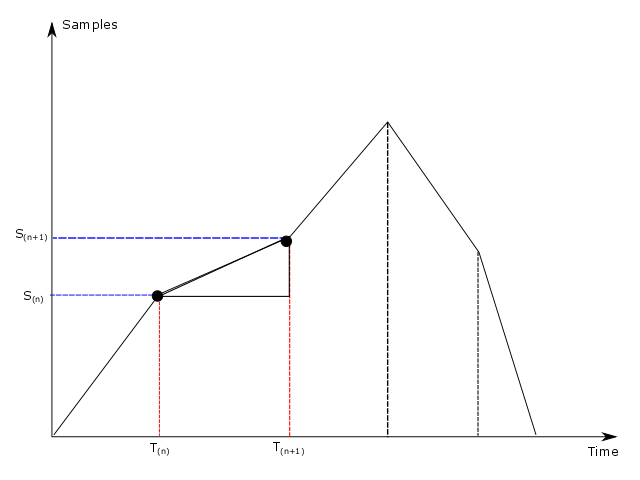
\includegraphics[width=0.75\columnwidth]{img/Q1_algorithm.png}
\end{center}
}
\vspace{20pt}
Graph of Samples vs. Time

Now, we know that the area under a section of the curve gives us the integral value of the function between the limits chosen.\\
Also, the slope of the curve between the two selected points gives us the differential value of the function between those two points.\\
This is shown in the figure marked by the red and blue lines.\\
The integral value between the two points marked in black is obtained by calculating the sum of the areas of the triangle and the rectangle below the points, as shown. The differential value is calculated by computing the value of $\frac{(y_2 - y_1)}{(x_2 - x_1)}$ where $(x_1,y_1)$ is the first point and $(x_2,y_2)$ is the second point.\\

Now, given the equation of the system as:
\begin{align}
M\ddot x(t) + \rho \dot x(t) + Kx(t) = F(t),\enspace t \ge 0\\
\shortintertext{We have}
M\ddot x(t) = F(t) - \rho \dot x - Kx
\end{align}
From the explanation above, it is clear that we cannot compute the value of $\ddot x(t)$. So,
\begin{align}
M\int_{t_1}^{t_2}\ddot x(t) = \int_{t_1}^{t_2} F(t) - \rho \int_{t_1}^{t_2} \dot x(t) - K \int_{t_1}^{t_2} x(t)\\
\implies M \{\dot x(t_2) - \dot x(t_1)\} = (t_2-t_1) - \rho \{x(t_2)-x(t_1)\} - K \int_{t_1}^{t_2} x(t)
\end{align}
Thus, the equation has been reduced to a set of three unknowns only, i.e. $M, K$ and $\rho$. The values of $\dot x(t), \int x(t)$ and $x(t)$ are calculated graphically, as described above.\\
Thus, given any four samples, using this algorithm, we obtain a set of three equations having three unknowns. Simultaneously solving the equations gives us values for the parameters $M, K$ and $\rho$.\\

Upon simulation in MATLAB, the values obtained were $M = 0.8988, K = 0.9152$ and $\rho = 0.0691$. This comes quite close to the actual values of the parameters, taken as $M = 1, K = 1, \rho = 0.1$.\\
\uuline{Thus, it is possible to determine approximately the values of $M, K$ and $\rho$ from an infinite list of samples.}
\end{homeworkSection}

\begin{homeworkSection}{(B)}
As demonstrated above, the algorithm requires at most 4 samples to determine the approximate values of $M, K$ and $\rho$. However, the higher the sampling rate, i.e. the more number of samples per unit time, the closer the algorithm approaches the true values of $M, K$ and $\rho$. Given a sufficiently high sampling rate, the error becomes negligible.
\end{homeworkSection}
\end{homeworkProblem}
\clearpage
%----------------------------------------------------------------------------------------
%	PROBLEM 2
%----------------------------------------------------------------------------------------

\begin{homeworkProblem}
\begin{homeworkSection}{(A)}
For the system given as:
\begin{align}
M\ddot x(t) + \rho \dot x(t) + Kx(t) = F(t),\enspace t \ge 0
\shortintertext{we have the following state-space equations}
\begin{bmatrix}
x\\ 
\dot x
\end{bmatrix}
=
\begin{bmatrix}
0 & 1\\
-\frac{K}{M} & -\frac{\rho}{M}
\end{bmatrix}
\begin{bmatrix}
x\\ 
\dot x
\end{bmatrix}
+
\begin{bmatrix}
0\\
1
\end{bmatrix}
F
\end{align}
This gives us the following state-space parameters:
\begin{align}
A =
\begin{bmatrix}
0 & 1\\
-\frac{K}{M} & -\frac{\rho}{M}
\end{bmatrix}\\
B = 
\begin{bmatrix}
0\\
1
\end{bmatrix}\\
C = 
\begin{bmatrix}
0 & 1
\end{bmatrix}\\
D = 0
\end{align}

For controllability, we have the following condition:
\begin{theorem}
A system is controllable if $\text{rank}[B\enspace AB\enspace A^B\enspace \dots \enspace A^{n-1}B] = n$
\end{theorem}
where $n$ is the order of the state.\\

In this particular case, the system is of order $n=2$. Thus,
\begin{align}
rank
\begin{bmatrix}
B & BA
\end{bmatrix}
=2\\
\implies
rank
\begin{bmatrix}
0 & 1\\
1 & -\frac{\rho}{M}
\end{bmatrix}
=2
\end{align}
Now, given this condition, we see that the controllability of the system does not depend on the value of $K$.\\
Also, irrespective of the value of $\rho$ or $M$, the rank of the matrix remains the same.\\
\uuline{Thus, for any value of $M,\rho$ and $K$, we have a system that is controllable.}
\end{homeworkSection}

\begin{homeworkSection}{(B)}
We are given the parameters as $M=1, \rho = 0.1, K=1$. Thus, we have:
\begin{align}
A = 
\begin{bmatrix}
0 & 1\\
-\frac{K}{M} & -\frac{\rho}{M}
\end{bmatrix}\\
\implies A = 
\begin{bmatrix}
0 & 1\\
-1 & -0.1
\end{bmatrix}
\shortintertext{We have the formula for $e^{At}$ as}
e^{At} = I + At + \frac{1}{2!} A^2 t^2 + \frac{1}{3!} A^3 t^3 + \dots\label{eqn:eAt}\\
\shortintertext{Solving for $A^2, A^3 \dots$ we have}
A=
\begin{bmatrix}
0 & 1\\
-1 & -0.1
\end{bmatrix}\\
A^2=
\begin{bmatrix}
-1 & -0.1\\
0.1 & -0.99
\end{bmatrix}\\
A^3=
\begin{bmatrix}
0.1 & -0.99\\
0.99 & 0.199
\end{bmatrix}\\
\vdots\nonumber\\
\shortintertext{We thus have:}
e^{At} =
\begin{bmatrix}
1 & 0\\
0 & 1
\end{bmatrix}
+
\begin{bmatrix}
0 & 1\\
-1 & -0.1
\end{bmatrix}t
+
\begin{bmatrix}
-0.5 & -0.05\\
0.05 & -0.495
\end{bmatrix}t^2
+
\begin{bmatrix}
0.0167 & -0.1650\\
0.1650 & 0.0332
\end{bmatrix}t^3
+ \dots
\end{align}
Now, the formula for calculating the unit step response is given by:
\begin{align}
y(t) = \int_{0}^{t_1} C e^{A(t_1-\tau)} B U(\tau) d\tau
\shortintertext{where $B$ and $C$ are parameters from the state-space given by:}
B = 
\begin{bmatrix}
0\\
1
\end{bmatrix}\\
C = 
\begin{bmatrix}
0 & 1
\end{bmatrix}
\shortintertext{$U(\tau)$ is the unit input, i.e. $1$ and $t_1$ is the upper limit of integration and $\tau$ is the time dependent variable.}\nonumber
\end{align}
Proceeding with these values, we expand the series given in Eqn.~\ref{eqn:eAt} to $20$ terms.\\
We get results as follows:\\

\problemAnswer{
\begin{center}
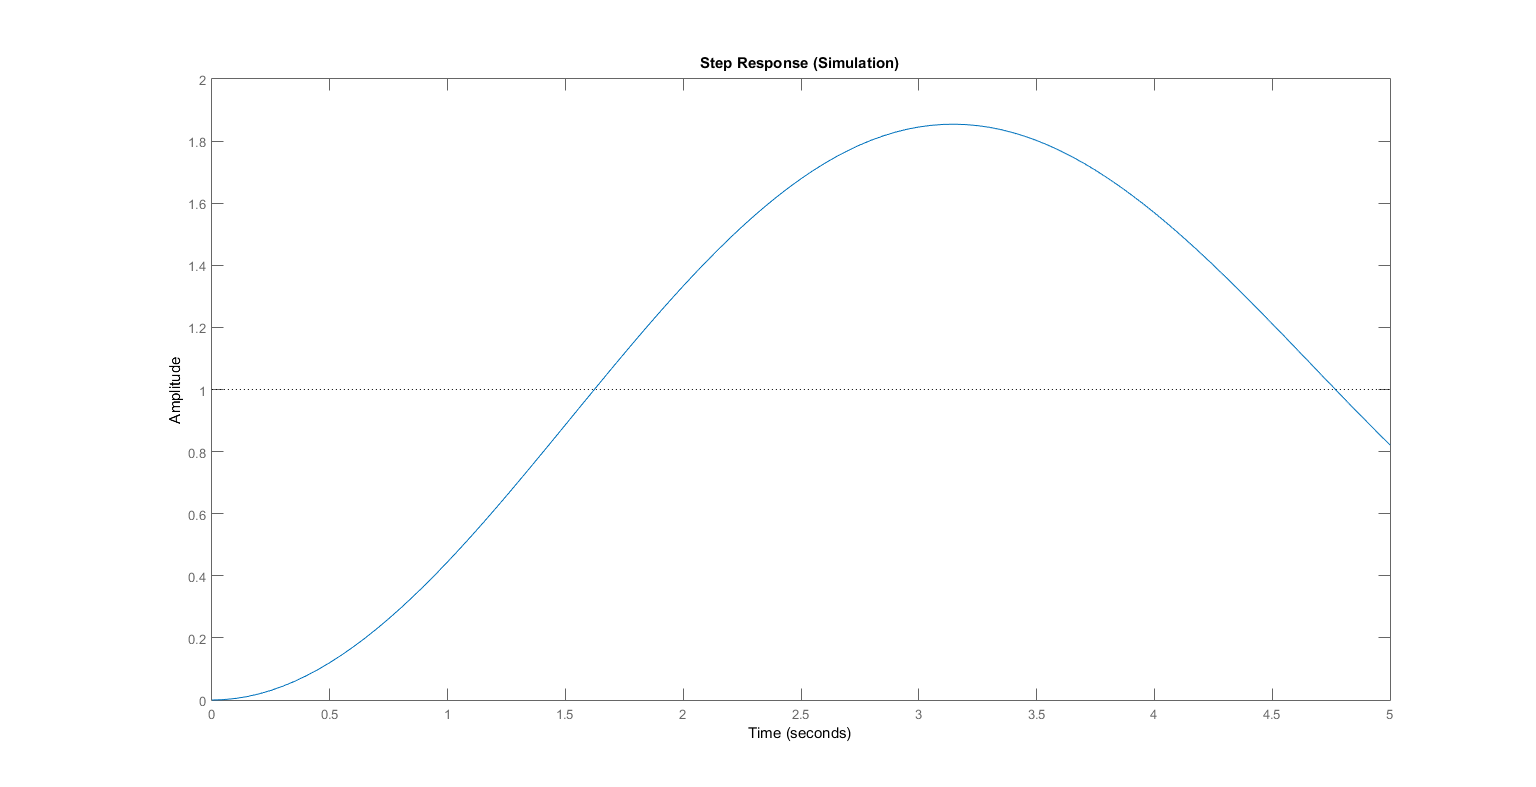
\includegraphics[width=0.9\columnwidth]{img/Q2B_simulation.png}
\end{center}
}
\vspace{20pt}
Simulated plot of unit step response of system

\problemAnswer{
\begin{center}
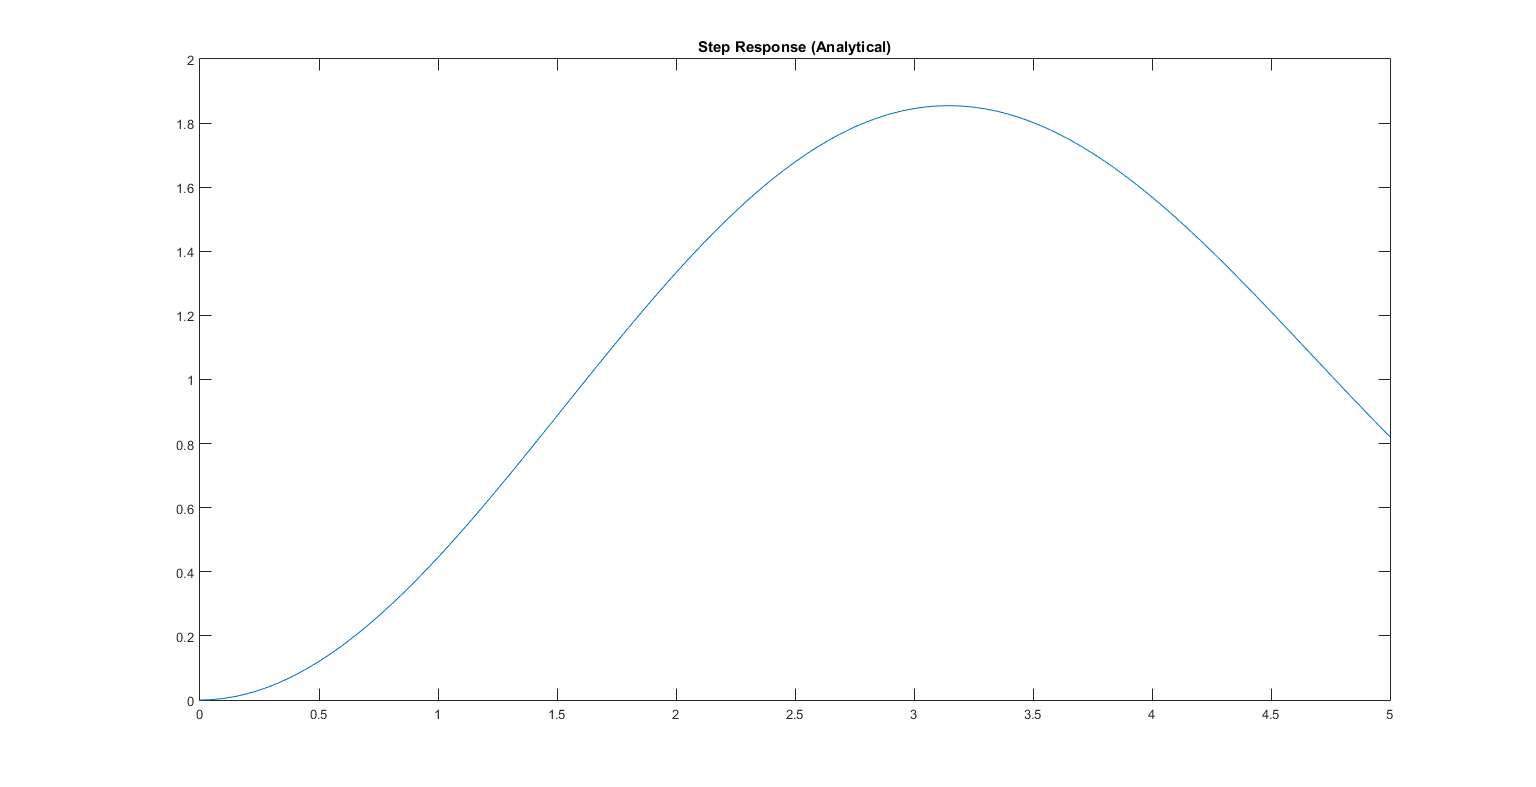
\includegraphics[width=0.9\columnwidth]{img/Q2B_analytical.png}
\end{center}
}
\vspace{20pt}
Analytical plot of unit step response of system

Following is the MATLAB code used to generate the plots:
\script{code/Q2B}{Unit Step Response Comparison}
\end{homeworkSection}

\begin{homeworkSection}{(C)}
We have the following equation for obtaining a control law:
\begin{align}
U(\tau) = B_k^T e^{A^T(t^* - \tau)} W_c(t^*,0)^{-1}(\vec{X_d}(t^*)-e^{At^*} \vec{X}(0))\\
\shortintertext{where $W_c(t^*,0)$ is the Controllability Gramian given by:}
W_c(t^*,0) = \int_{0}^{t^*} e^{A\gamma} B_k B^T_k e^{A^T \gamma} d\gamma
\end{align}
We are given the following values:
\begin{align}
M = 1\nonumber\\
K = 1\nonumber\\
\rho = 0.1\nonumber\\
\vec{X}(0) = 1\nonumber\\
\vec{X_d}(t^*) = 0\nonumber\\
t^* = 10\nonumber
\end{align}
Computing $U(\tau)$ using MATLAB, we obtain:
\begin{spverbatim}
(1.07e+18*cos(399^(1/2)*(tau/20 - 1/2))*exp(tau/20 + 1/2) +
92.41e+15*cos(399^(1/2)*(tau/20 + 1/2))*exp(tau/20 + 1/2) -
1.16e+18*cos(399^(1/2)*(tau/20 - 1/2))*exp(tau/20 + 3/2) + 
95.33e+15*399^(1/2)*exp(tau/20 + 1/2)*
sin(399^(1/2)*(tau/20 - 1/2))+2.91e+15*399^(1/2)*
exp(tau/20 + 1/2)*sin(399^(1/2)*(tau/20 + 1/2)) -
98.25e+15*399^(1/2)*exp(tau/20 + 3/2)*sin(399^(1/2)*
(tau/20 - 1/2)))/(45.03e+15*(399*exp(2) - 800*exp(1) + 
2*exp(1)*cos(399^(1/2)) + 399)), -(3.69e+18*cos(399^(1/2)*
(tau/20 - 1/2))*exp(tau/20 + 1/2) - 125.6e+15*cos(399^(1/2)*
(tau/20 + 1/2))*exp(tau/20 + 1/2) - 3.57e+18*cos(399^(1/2)*
(tau/20 - 1/2))*exp(tau/20 + 3/2) - 116.72e+15*399^(1/2)*
exp(tau/20 + 1/2)*sin(399^(1/2)*(tau/20 - 1/2)) + 8.94e+15*399^(1/2)*
exp(tau/20 + 1/2)*sin(399^(1/2)*(tau/20 + 1/2)) + 107.77e+15*399^(1/2)*
exp(tau/20 + 3/2)*sin(399^(1/2)*(tau/20 - 1/2)))/
(90.07e+15*(399*exp(2) - 800*
exp(1) + 2*exp(1)*cos(399^(1/2)) + 399))
\end{spverbatim}
\newline
To prove that the control law works as expected, following is the scope output when the above function is given as input to the state-space with a time varying value of $\tau$:\\
\problemAnswer{
\begin{center}
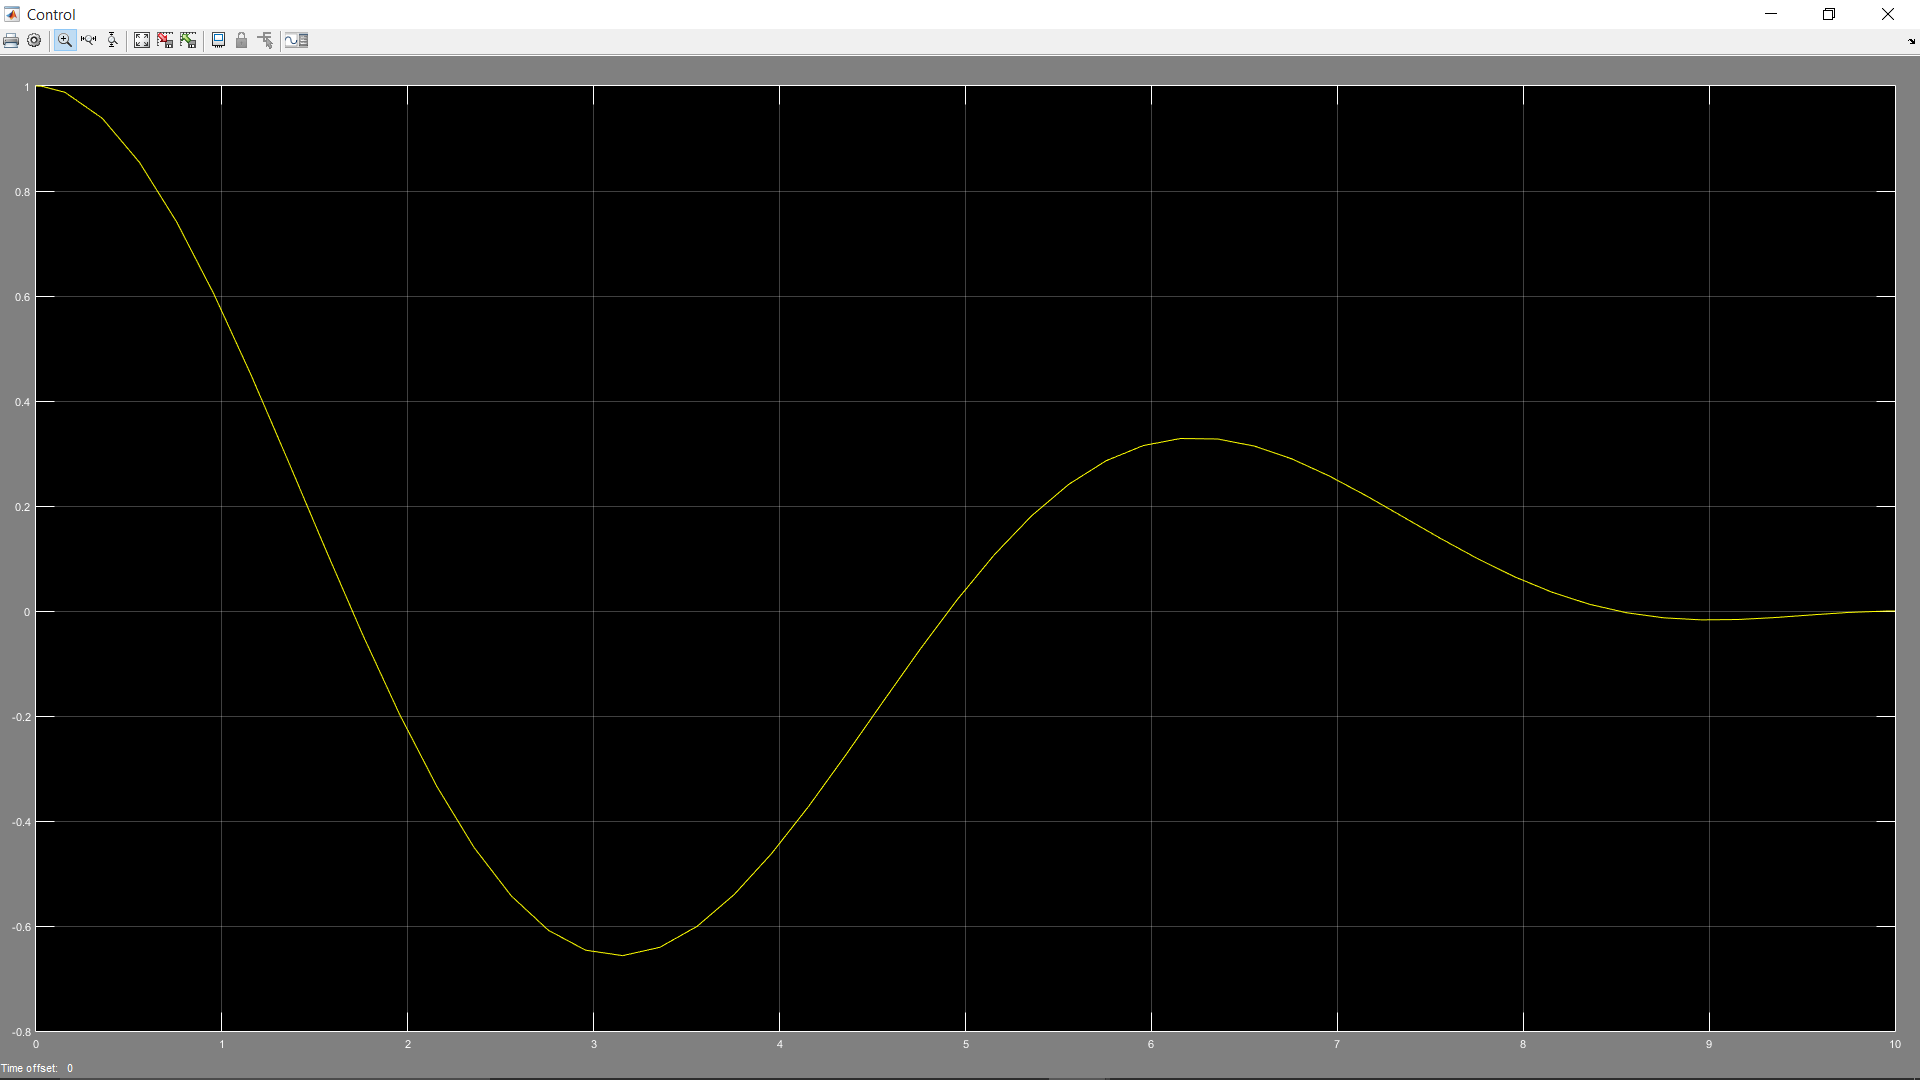
\includegraphics[width=1.0\columnwidth]{img/Q2C_controlCheck.png}
\end{center}
}
\vspace{20pt}
Verifying Control Output $U(t)$

We can see that the state goes from $1$ to $0$ and converges at time $t \geq 10$, which is the desired output.
\end{homeworkSection}
\end{homeworkProblem}

%----------------------------------------------------------------------------------------
%	PROBLEM 3
%----------------------------------------------------------------------------------------

\begin{homeworkProblem}
\begin{homeworkSection}{(A)}
\problemAnswer{
\begin{center}
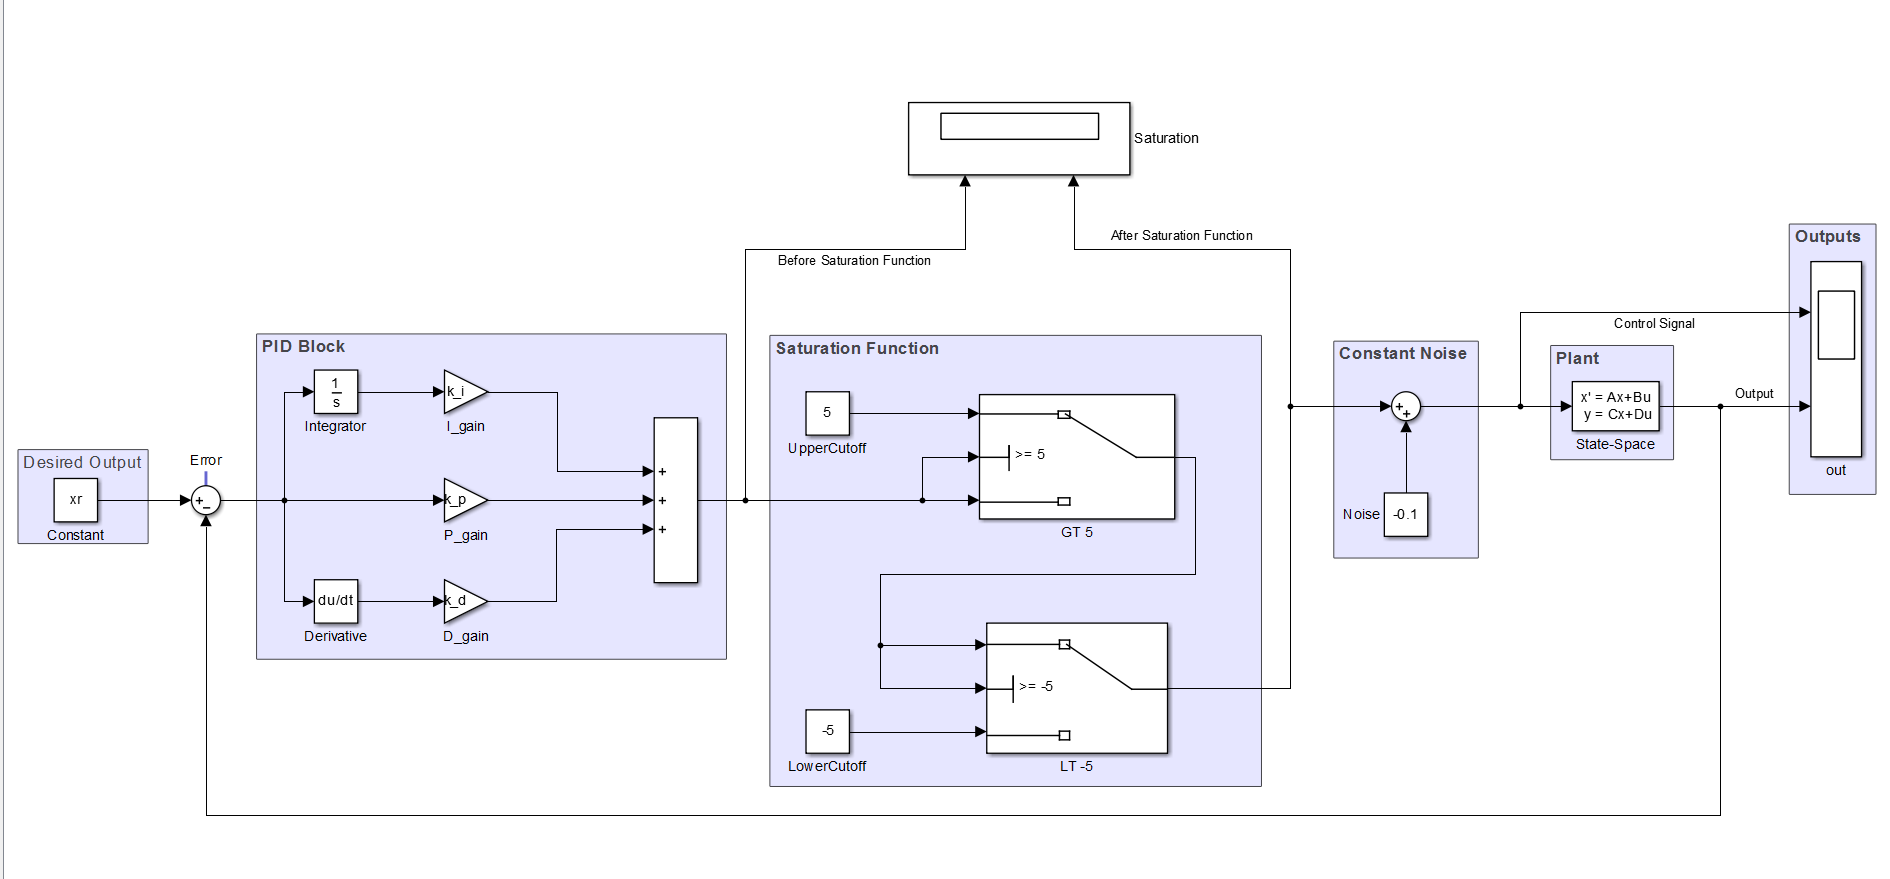
\includegraphics[width=1.0\columnwidth]{img/Q3A_PID.png}
\end{center}
}
\vspace{20pt}
The PID Controller Design

It is given in the problem statement that $M=1, K=1$ and $\rho = 0.1$. We create our state-space using these parameters.\\
Also given is that $x(0) = \dot x(0) = 0$, which is set in the state-space block. We also have $-0.1 <F_d <0.1$, which is a known, constant disturbance as shown in the `Constant Noise' panel of the diagram.\\
Also shown is the `Saturation Function' block, which is used to satisfy the condition that $F(t)$ saturates at $|F(t)| \geq 5$.

Assuming a reference value $x_r = 4$ and $k_P = 0.5, k_I = 0.6, k_D = 1.6$ as the PID gain values, we get the following output:\\
\problemAnswer{
\begin{center}
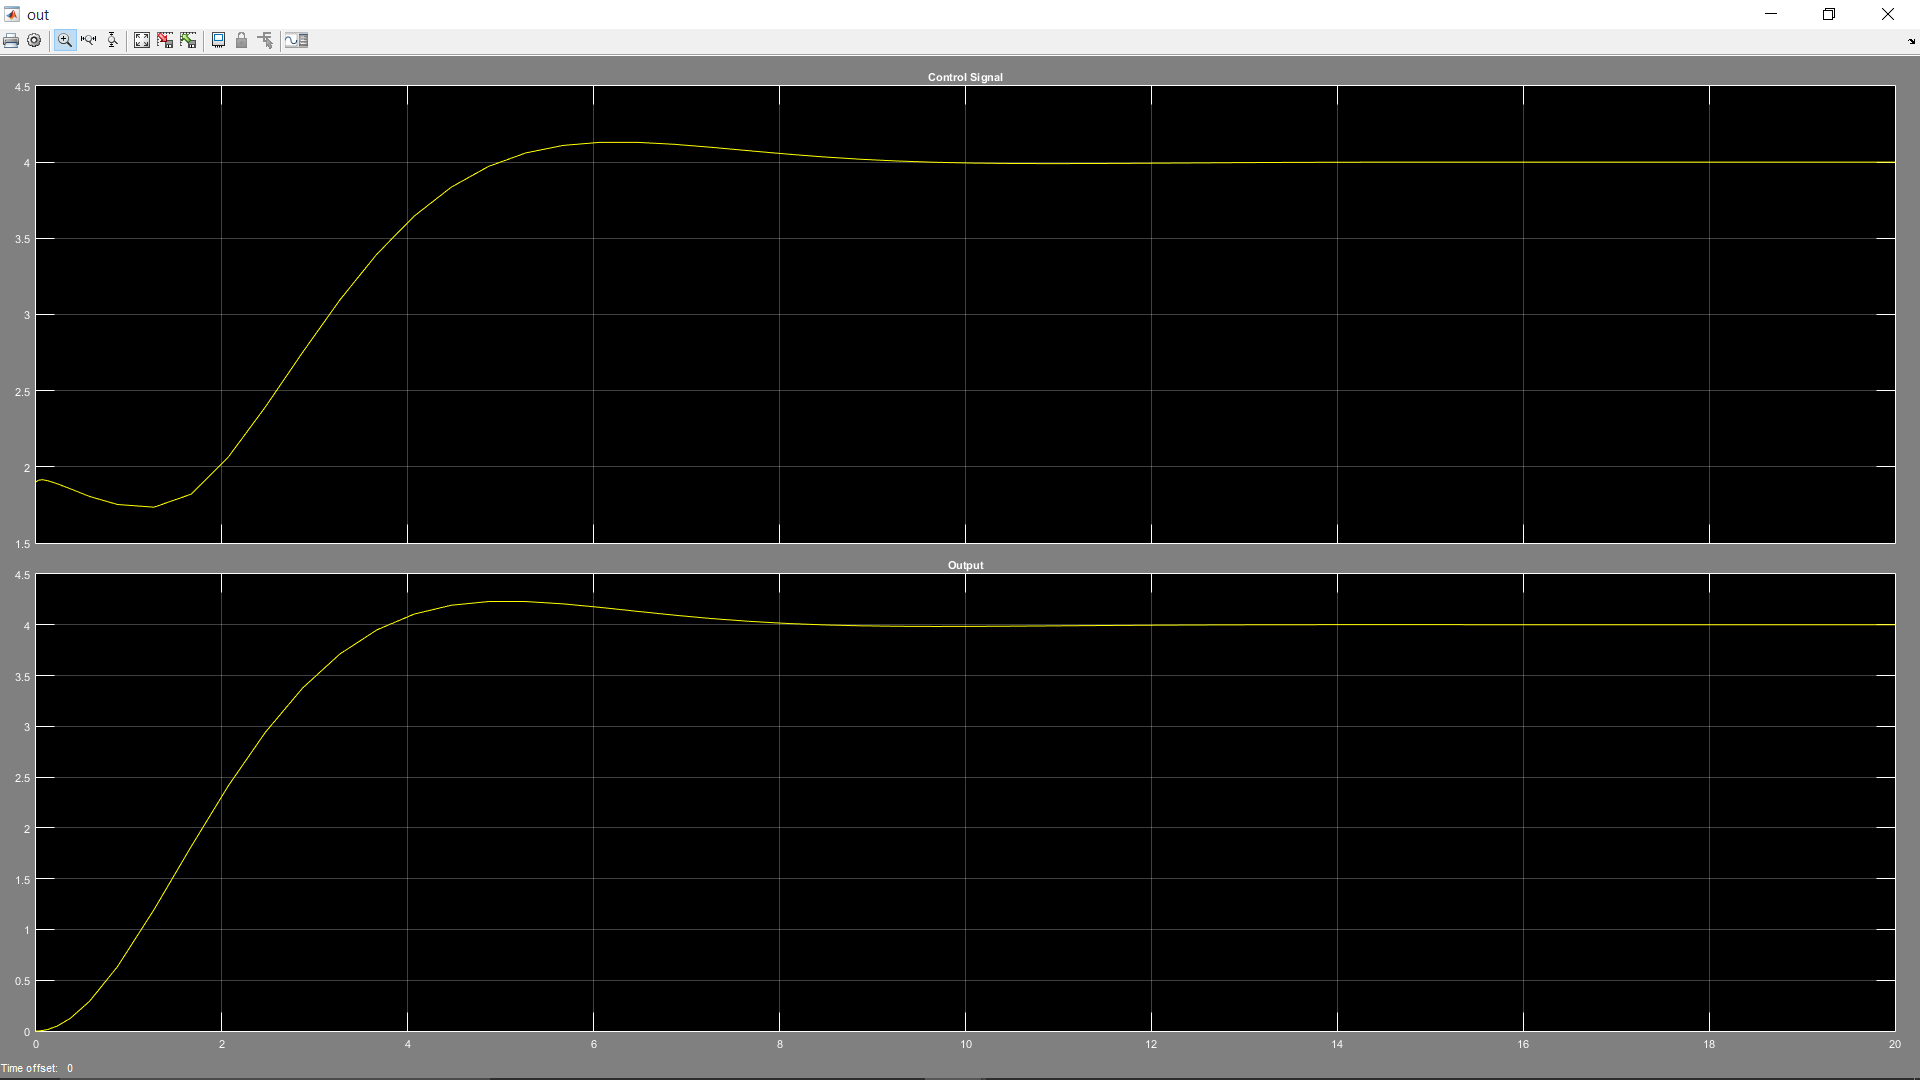
\includegraphics[width=1.0\columnwidth]{img/Q3A_noSaturatePID.png}
\end{center}
}
\vspace{20pt}
Tracking with zero asymptotic error

For a design for $F(t)$ which never saturates, $k_P = 0.5, k_I = 0.6, k_D = 1.6$ were selected as the PID gain values. A comparison of scope outputs before and after the `Saturation Function' block is shown. They are the same outputs, proving that no saturation/cutoff was done.\\
\problemAnswer{
\begin{center}
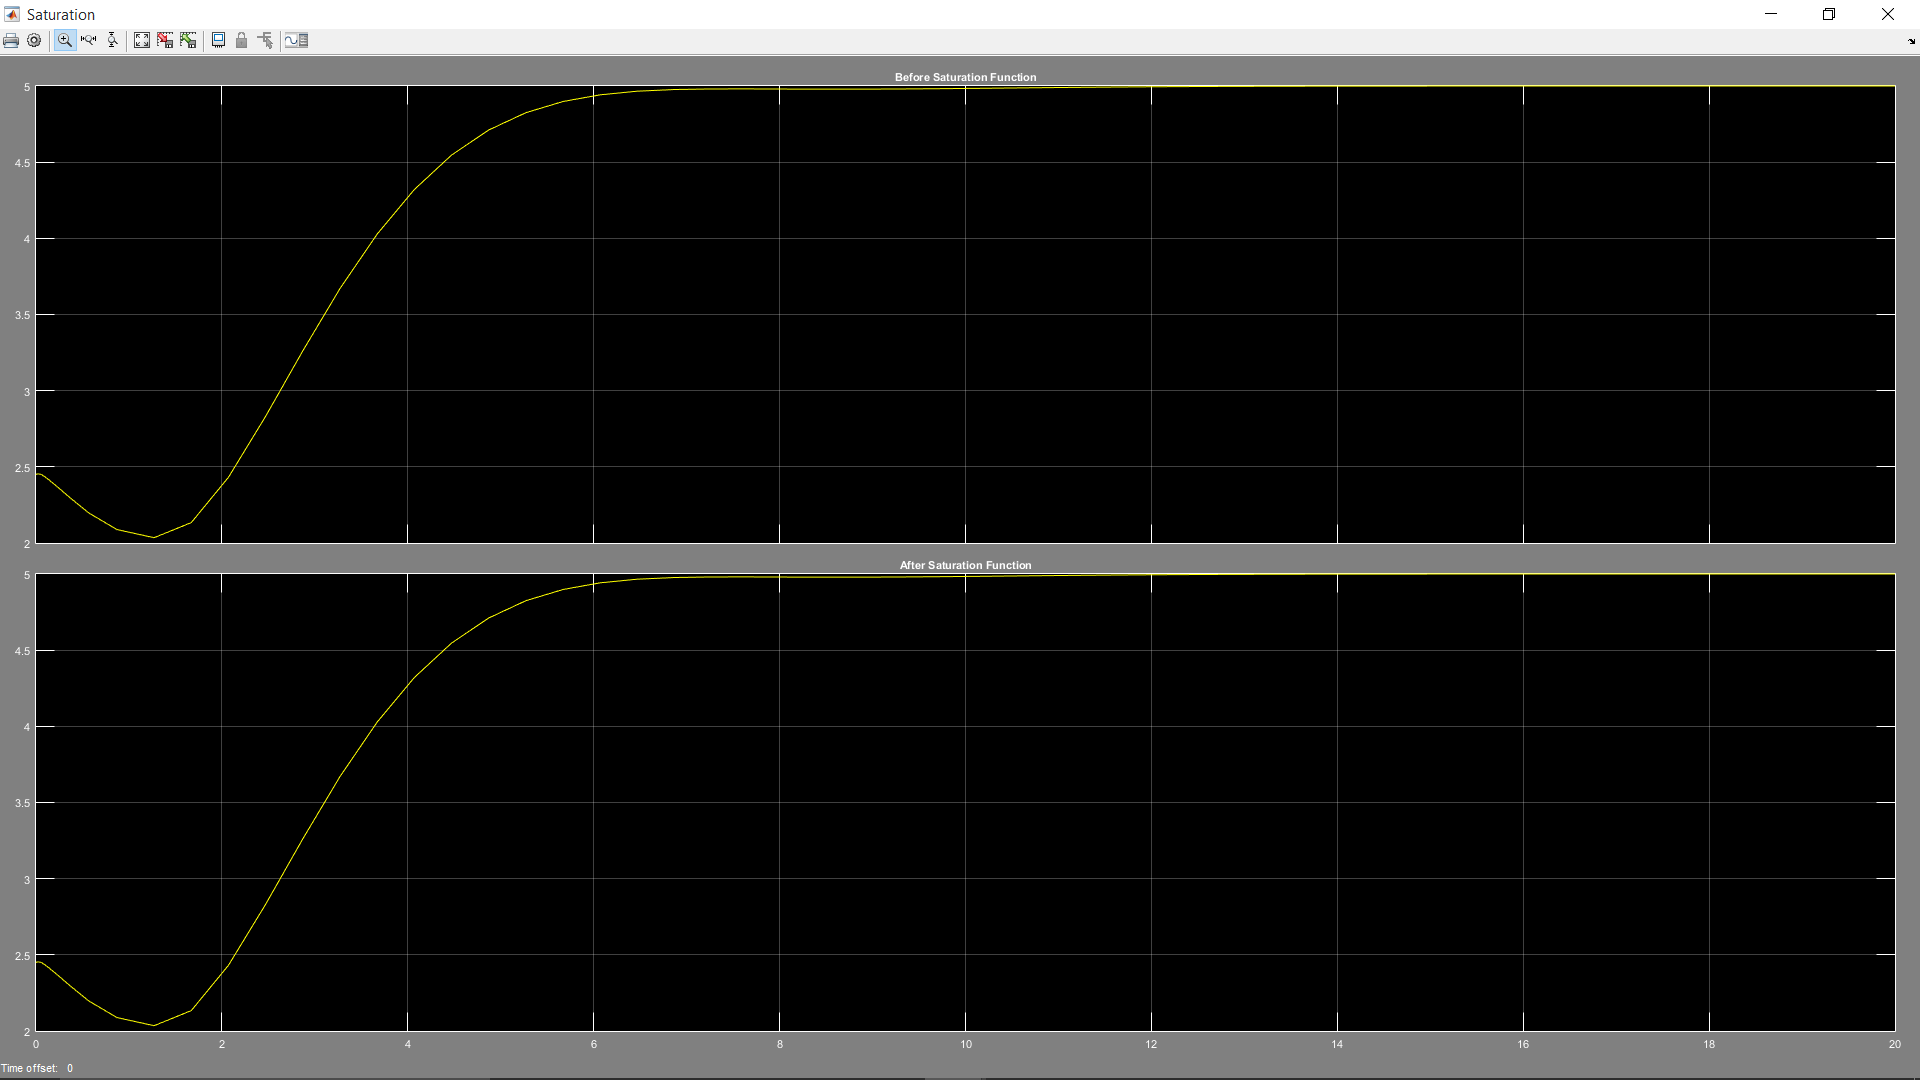
\includegraphics[width=1.0\columnwidth]{img/Q3A_noSaturate.png}
\end{center}
}
\vspace{20pt}
No Saturation of $F(t)$

In order to show saturation, $k_P = 5, k_I = 1, k_D = 1$ were selected as the PID gain values. A similar comparison of scope outputs before and after the `Saturation Function' block is shown. It is clear from the graph that any value above $5$ and below $-5$ is cutoff, thus showing that saturation occurred.\\
\problemAnswer{
\begin{center}
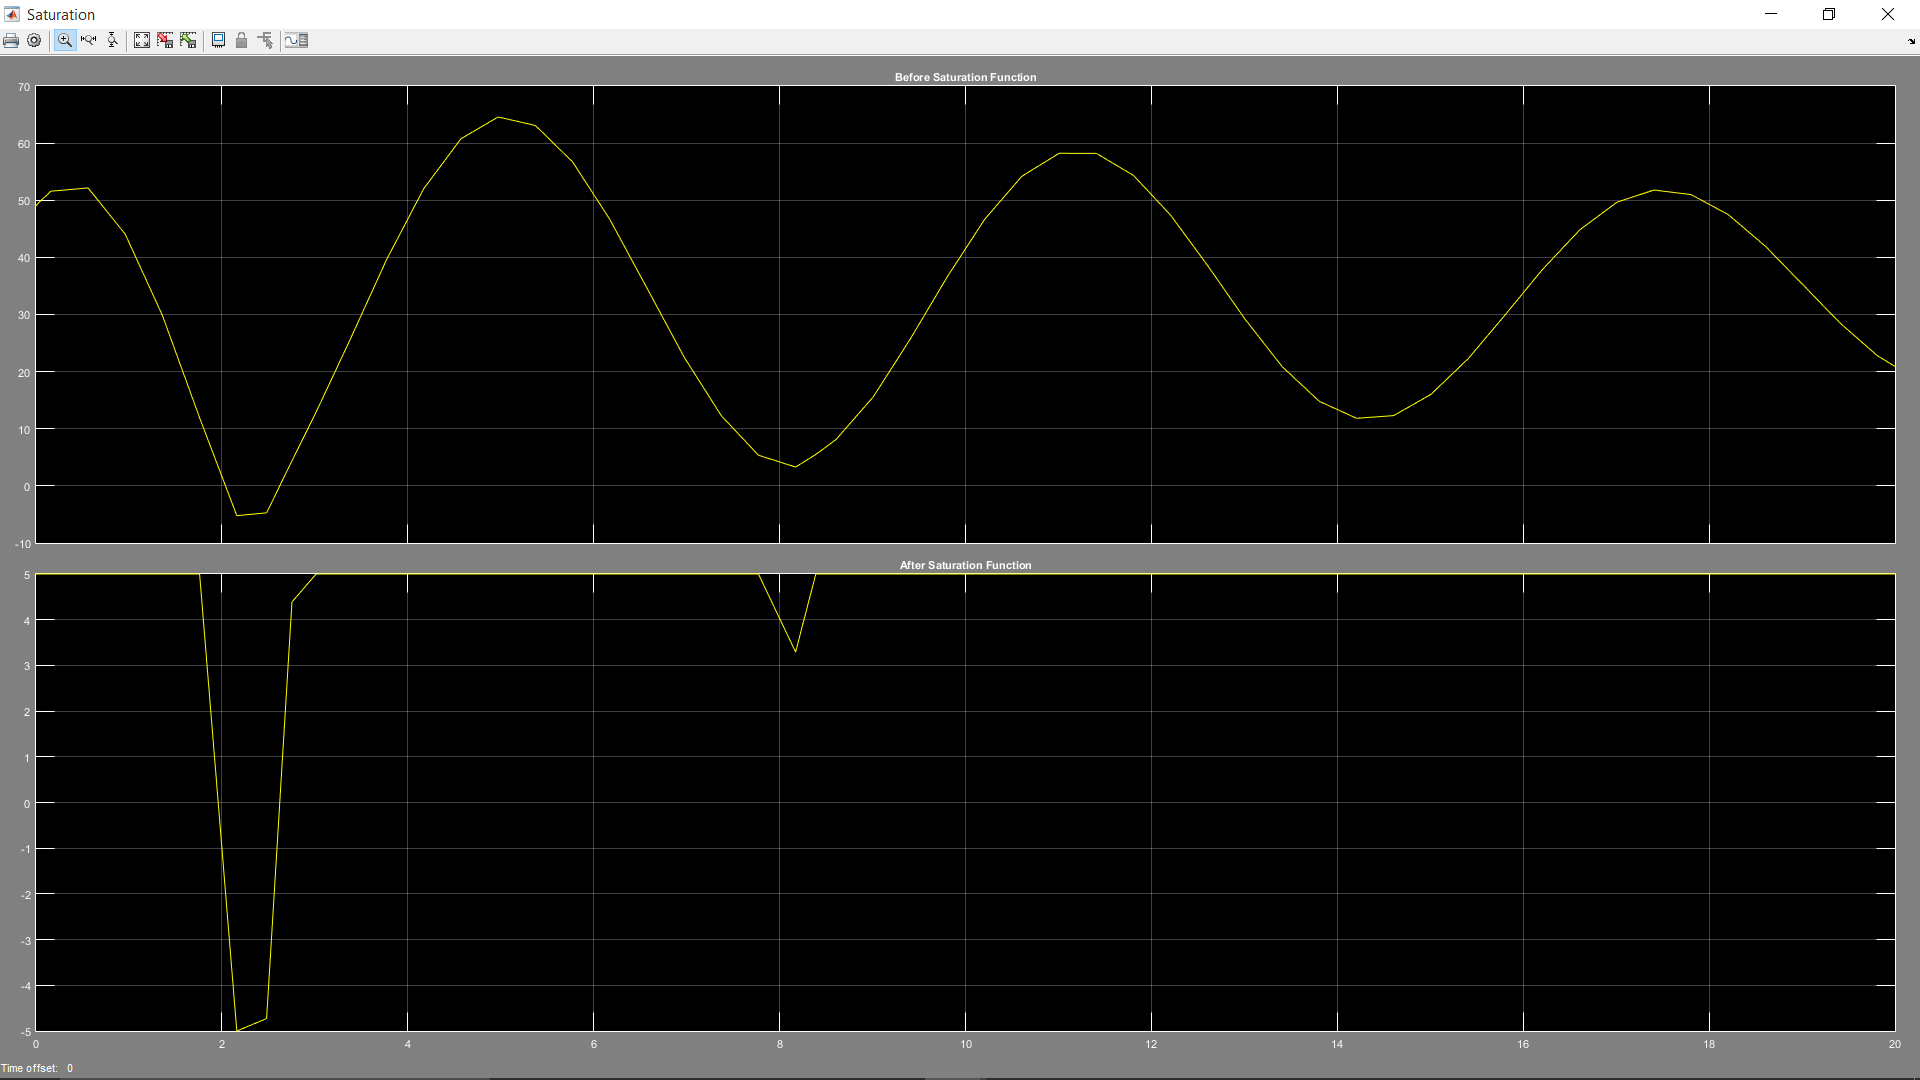
\includegraphics[width=1.0\columnwidth]{img/Q3A_saturate.png}
\end{center}
}
\vspace{20pt}
Saturation of $F(t)$

The output of the system is shown below:\\
\problemAnswer{
\begin{center}
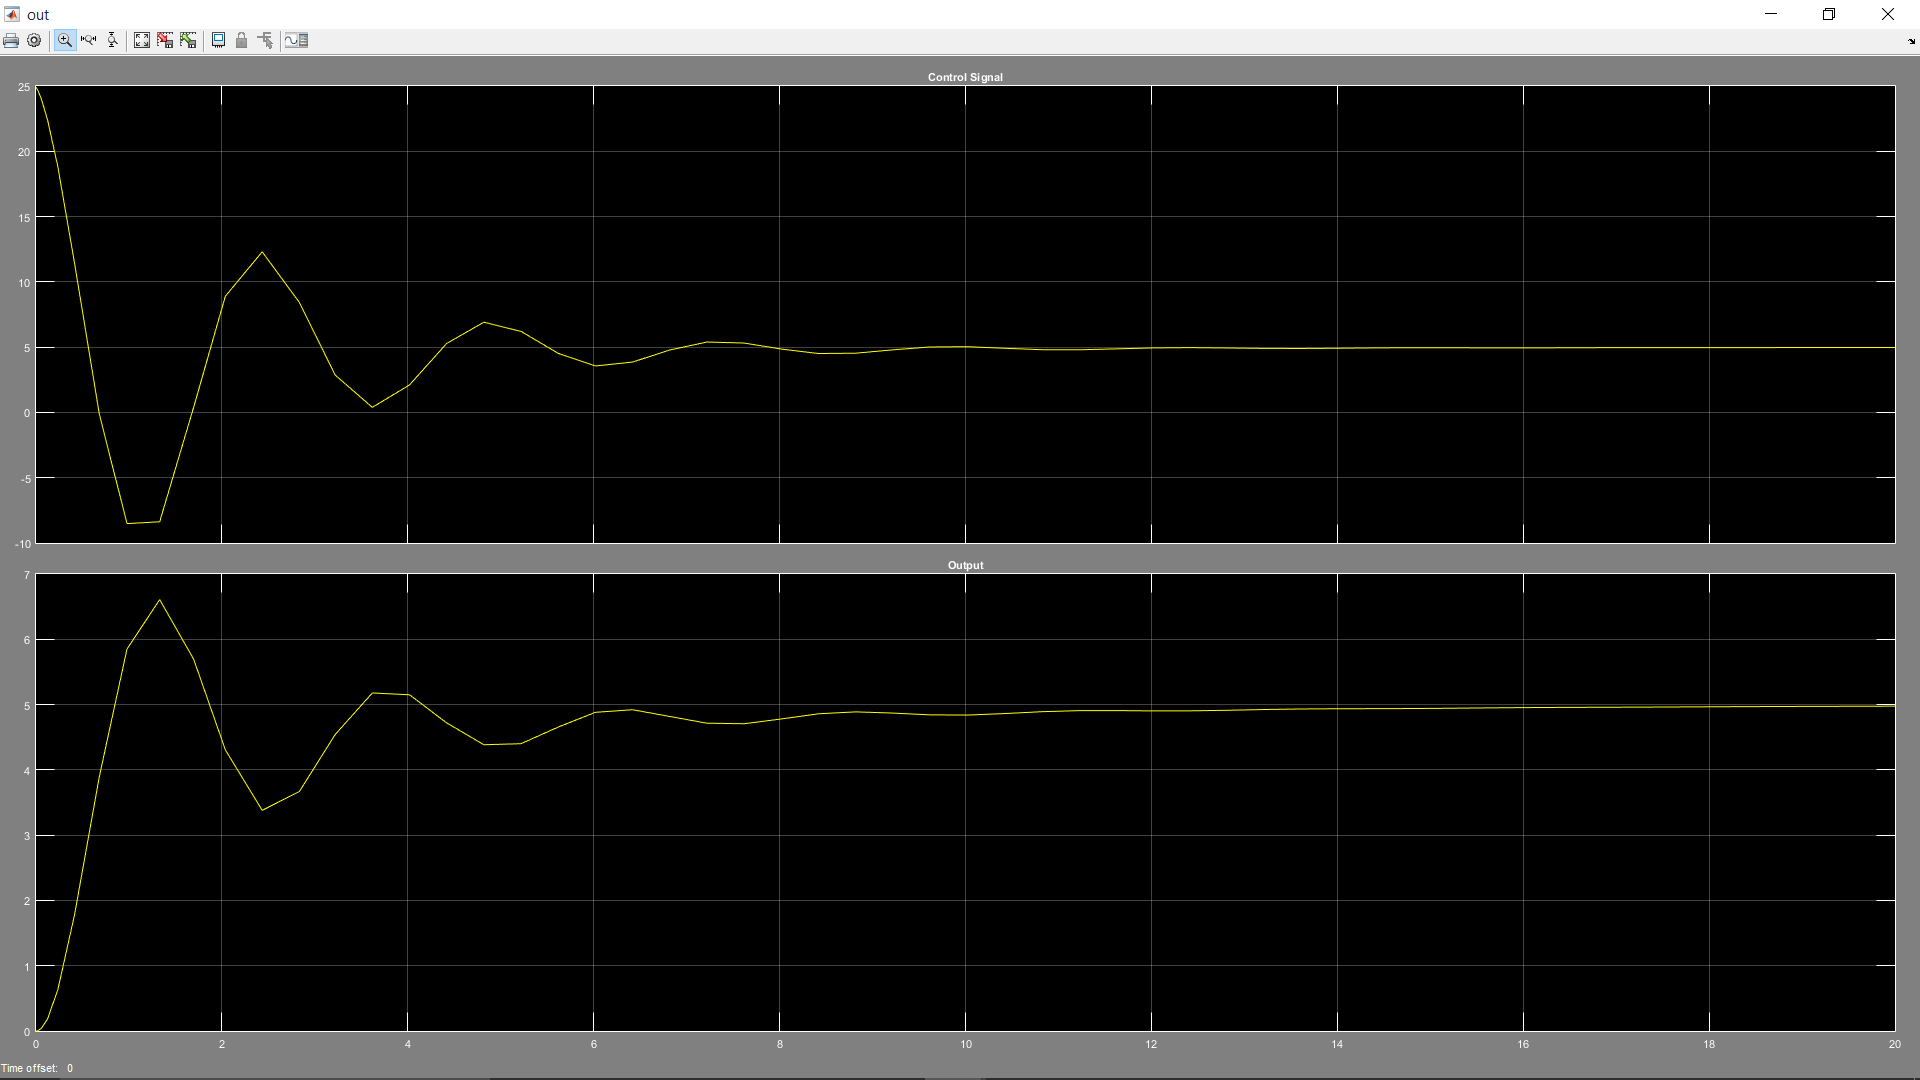
\includegraphics[width=1.0\columnwidth]{img/Q3A_saturatePID.png}
\end{center}
}
\vspace{20pt}
Output with saturation of $F(t)$
\end{homeworkSection}

\begin{homeworkSection}{(B)}
Ignoring the saturation condition that $F(t)$ saturates at $|F(t)| \geq 5$, we choose the following state variables for the PID system:
\begin{align}
X =
\begin{bmatrix}
x(t) & \dot x(t) & \epsilon
\end{bmatrix}\\
U = x_r(t)
\shortintertext{where $\epsilon = \int_{0}^{t}(x_r-x(t))dt$ is the tracking error and $x_r(t)$ is the desired output.}
\end{align}

The system is defined by
\begin{align}
M\ddot x(t) + \rho \dot x(t) + Kx(t) = F(t)\\
\implies M\ddot x(t) = F(t)  - \rho \dot x(t) - Kx(t)\label{eqn:M}
\end{align}

We have the general formula for control signal from a PID controller as:
\begin{align}
F(t) = k_P(x_r-x(t)) - k_D \dot x(t) + k_I \epsilon_I - Kx(t) - \rho \dot x(t)\label{eqn:F}
\end{align}
Substituting Eqn.~\ref{eqn:F} in Eqn.~\ref{eqn:M}, we get:
\begin{align}
M\ddot x(t) = k_P x_r - (k_P + K) x(t) - (k_D + \rho)\dot x(t) + k_I \epsilon_I\\
\shortintertext{The general equation for state-space is given by:}
\mathbf{\dot X} = \mathbf{A}X + \mathbf{B}U\label{eqn:genX}\\
\shortintertext{So, we have}
\dot X = 
\begin{bmatrix}
0 & 1 & 0\\
\frac{-(K+k_P)}{M} & \frac{-(k_D + \rho)}{M} & \frac{(k_I}{M}\\
-1 & 0 & 0
\end{bmatrix}X
+
\begin{bmatrix}
0\\
\frac{(k_P)}{M}\\
1
\end{bmatrix}U\\
\shortintertext{Comparing the above with Eqn.~\ref{eqn:genX}, we get}
A=
\begin{bmatrix}
0 & 1 & 0\\
\frac{-(K+k_P)}{M} & \frac{-(k_D + \rho)}{M} & \frac{(k_I}{M}\\
-1 & 0 & 0
\end{bmatrix}\\
B=
\begin{bmatrix}
0\\
\frac{(k_P)}{M}\\
1
\end{bmatrix}
\end{align}
This gives us the state-space representation of the closed loop system.\\
We now check for stability using the following condition:
\begin{theorem}
For a stable system, the eigenvalues of $A$ must have a negative real part.
\end{theorem}
To calculate the eigenvalues, we have:
\begin{align}
|\lambda I - A| = 0\\
\implies \lambda \Bigg[ \lambda^2 + \frac{k_D + \rho}{M} \lambda \Bigg] + \lambda \frac{k_P + K}{M} + \frac{k_I}{M} = 0\\
\shortintertext{Considering $k_P = 1.5, k_I = 2, k_D = 1.6$ as the PID gain values, we get}
\lambda \Bigg[ \lambda^2 + \frac{1.6 + 0.1}{1} \lambda \Bigg] + \lambda \frac{1.5 + 1}{1} + \frac{2}{1} = 0\\
\implies \lambda^3 + 1.7 \lambda^2 + 2.5 \lambda + 2 = 0
\end{align}
The roots for above polynomial are:
\begin{align}
-0.3051 + 1.3198i\nonumber\\
-0.3051 - 1.3198i\nonumber\\
-1.0899 + 0.0000i\nonumber
\end{align}
It is clear from the eigenvalues that all of them have negative real parts. Thus, we conclude that the system is stable.\\
\problemAnswer{
\begin{center}
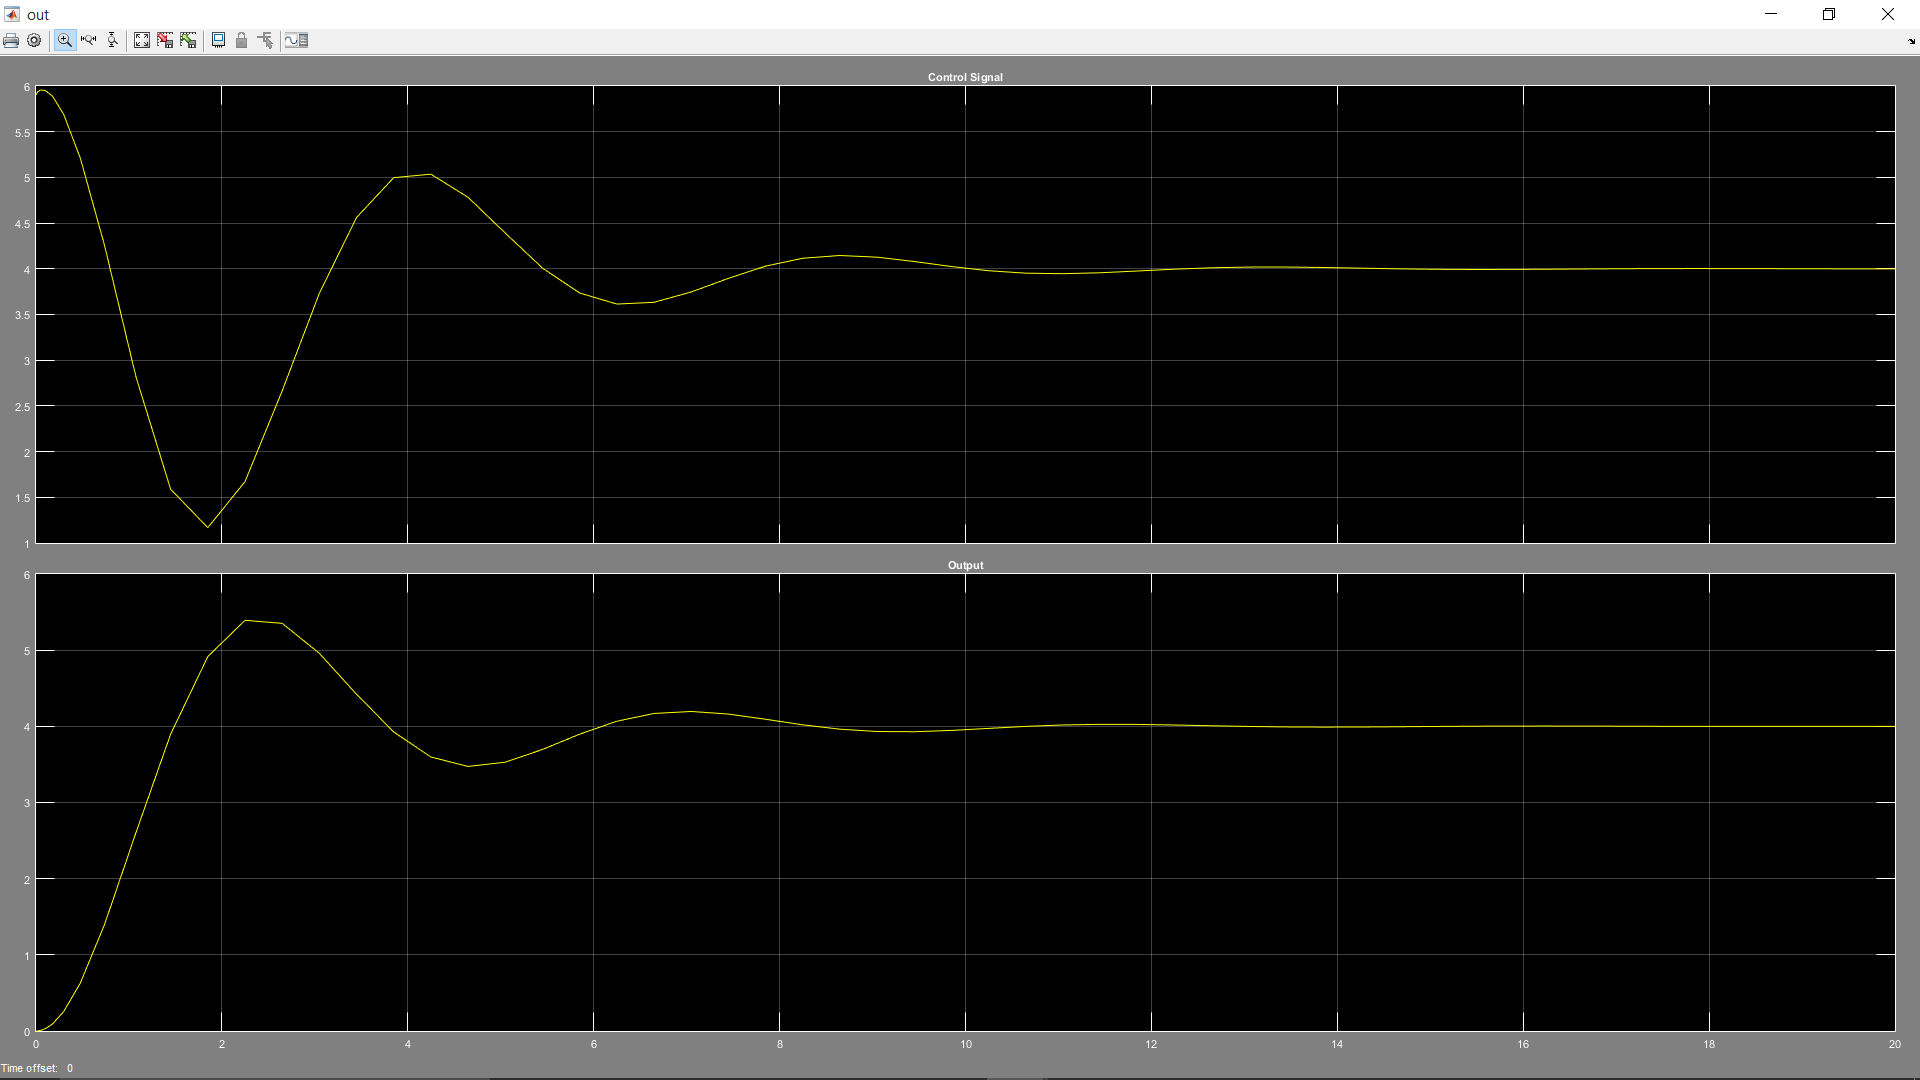
\includegraphics[width=1.0\columnwidth]{img/Q3B_stable.png}
\end{center}
}
\vspace{20pt}
Stable output taking $k_P = 1.5, k_I = 2, k_D = 1.6$ as PID gains

Common intuition might dictate that if a system without PID control is stable, i.e. the $A$ matrix has eigenvalues having negative real parts, it would remain stable even if a PID controller is added, i.e. the $A$ matrix is augmented with the error $\epsilon$. The naive assumption might be that the gain values of the PID controller are independent of the original state-space parameters.\\
However, the tracking error $\epsilon$ is directly affected by the PID gain values, which in turn affects the output of the system since there is a feedback loop. Thus, it is possible to choose values of $k_P, k_I$ and $k_D$ such that the system becomes unstable, even though it was originally a stable system.
\newline

\hrulefill\\
Considering a PID controller system without a `Saturation Function', we take  $k_P = 5, k_I = 0, k_D = -5$ as the gain values. The scope output below shows a closed loop system with saturated $F(t)$ giving an unstable output.\\
\problemAnswer{
\begin{center}
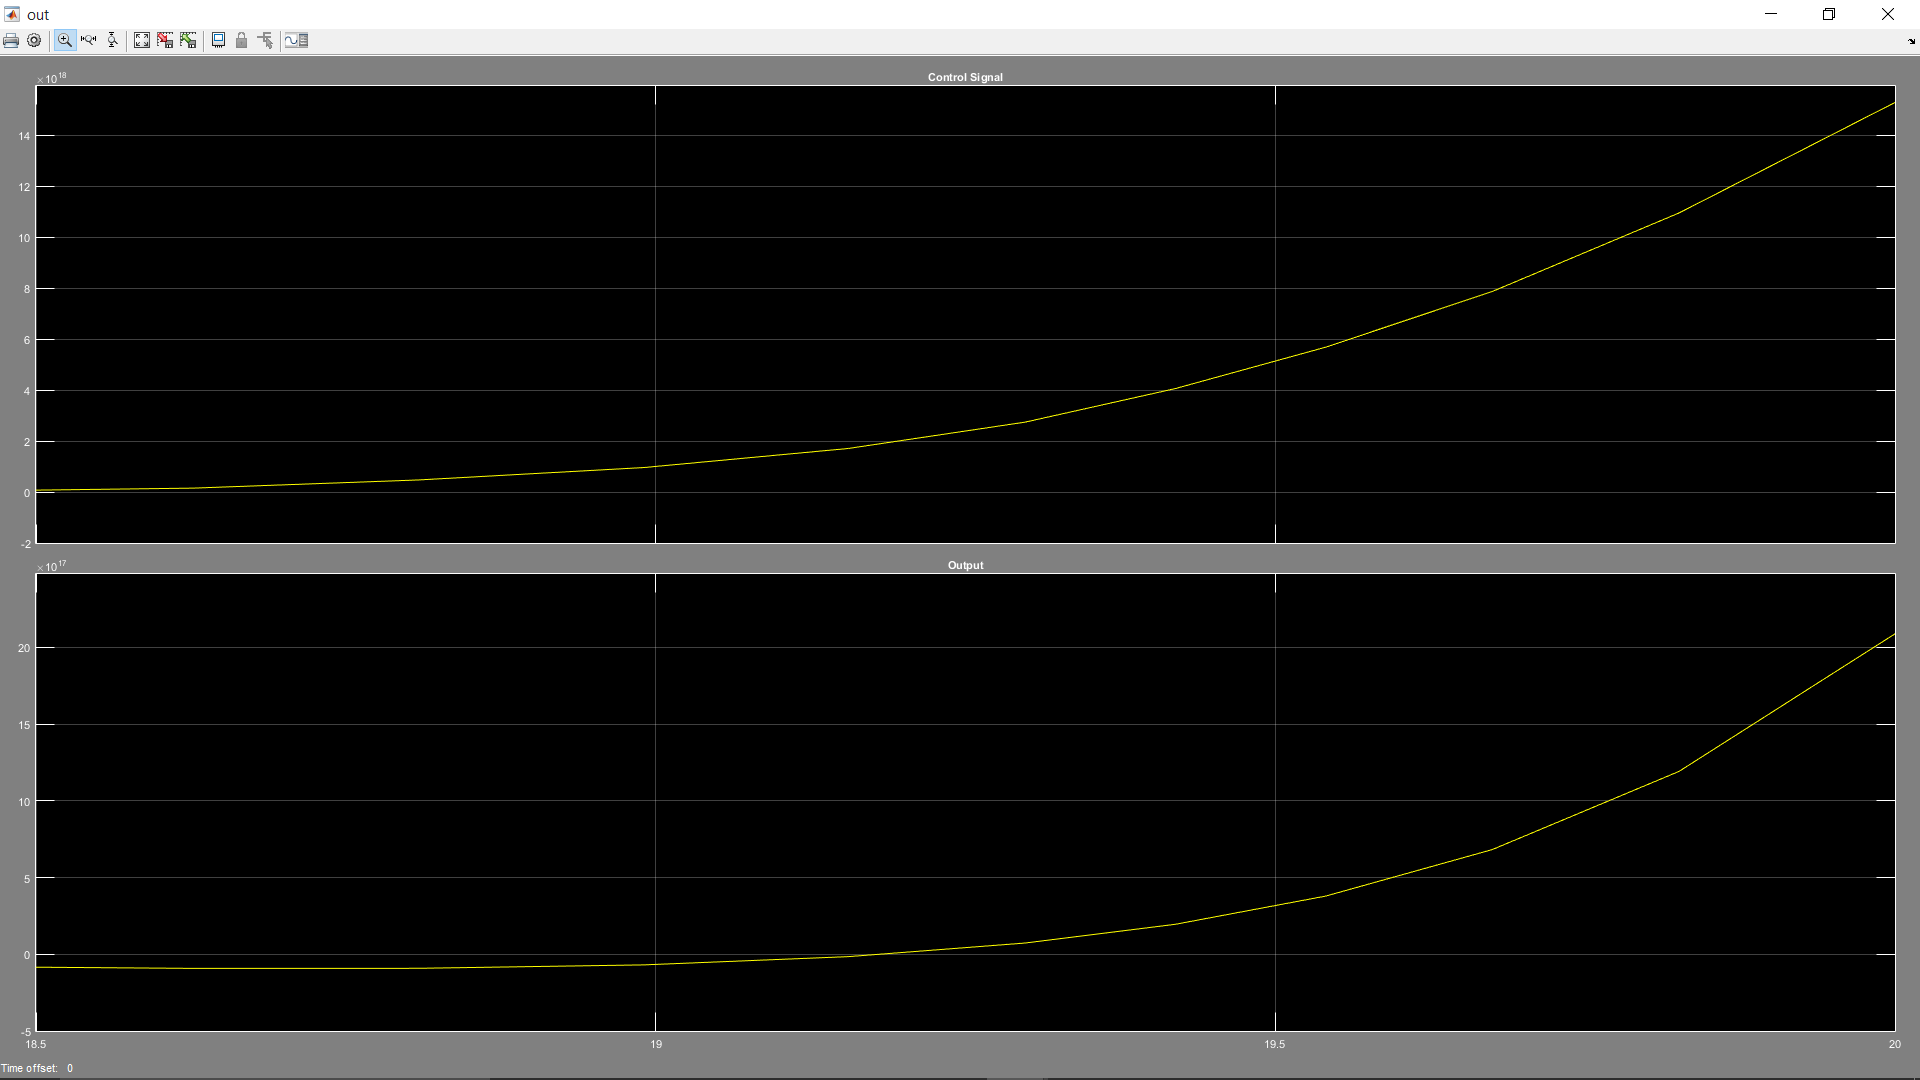
\includegraphics[width=1.0\columnwidth]{img/Q3B_unstable.png}
\end{center}
}
\vspace{20pt}
Saturated $F(t)$ with unstable output
\end{homeworkSection}
\end{homeworkProblem}
\clearpage

%----------------------------------------------------------------------------------------
%	PROBLEM 4
%----------------------------------------------------------------------------------------

\begin{homeworkProblem}
\begin{homeworkSection}{Q. 6-18}
From the problem statement, we are given the following simplified equations of motion:
\begin{align}
J_1\ddot q_1 = \tau\label{eqn:init1}\\
J_2\ddot q_2 = \tau\label{eqn:init2}
\end{align}
For this system of $2^{nd}$ order equations, we choose the input variables as follows:
\begin{align}
x_1 = q_1\\
x_2 = \dot q_1\\
x_3 = q_2\\
x_4 = \dot q_2\\
\implies X = 
\begin{bmatrix}
q_1 & \dot q_1 & q_2 & \dot q_2
\end{bmatrix}
\end{align}
Also, assuming $\tau$ as input, we have the following output variables:
\begin{align}
q_1\\
q_2\\
\implies Y = 
\begin{bmatrix}
q_1 & q_2
\end{bmatrix}
\end{align}
The general equations for state-space is given as follows:
\begin{align}
\mathbf{\dot X} = \mathbf{A}X + \mathbf{B}U\label{eqn:x}\\ 
\mathbf{Y} = \mathbf{C}X + \mathbf{D}U \label{eqn:y}
\end{align}
So, we have 
\begin{align}
\dot X =
\Bigg\{ \begin{bmatrix}
A_{11} & A_{12} & A_{13} & A_{14}\\
A_{21} & A_{22} & A_{23} & A_{24}\\
A_{31} & A_{32} & A_{33} & A_{34}\\
A_{41} & A_{42} & A_{43} & A_{44}\\
\end{bmatrix}
\times X \Bigg\}
+
\Bigg\{ \begin{bmatrix}
B_{11}\\B_{21}\\B_{31}\\B_{34}
\end{bmatrix}
\times U \Bigg\} 
\end{align}
Thus, we need to select values of $[A_{11}\dots A_{44}]$ and $[B_{11}\dots B_{41}]$ such that Eqn. \ref{eqn:AB} is satisfied.\\
So, from Eqn. \ref{eqn:x} we have:
\begin{align}
\dot X = 
\Bigg\{ \begin{bmatrix}
0 & 1 & 0 & 0\\
0 & 0 & 0 & 0\\
0 & 0 & 0 & 1\\
0 & 0 & 0 & 0\\
\end{bmatrix}
\times 
\begin{bmatrix}
q_1\\\dot q_1\\q_2\\\dot q_2
\end{bmatrix}
\Bigg\}
+
\Bigg\{ \begin{bmatrix}
0\\\frac{1}{J_1}\\0\\\frac{1}{J_2}
\end{bmatrix}
\times \tau
\Bigg\} \label{eqn:AB}
\end{align}

Similarly, from Eqn. \ref{eqn:y} we get:
\begin{align}
Y = 
\Bigg\{ \begin{bmatrix}
1 & 0 & 0 & 0\\
0 & 0 & 1 & 0\\
\end{bmatrix}
\times 
\begin{bmatrix}
q_1\\\dot q_1\\q_2\\\dot q_2
\end{bmatrix}
\Bigg\}
+
\Bigg\{ 0 \times \tau
\Bigg\}\label{eqn:CD}
\end{align}

Thus, from Eqns.~\ref{eqn:AB} and \ref{eqn:CD}, we get the values of:
\begin{align}
A = 
\begin{bmatrix}
0 & 1 & 0 & 0\\
0 & 0 & 0 & 0\\
0 & 0 & 0 & 1\\
0 & 0 & 0 & 0
\end{bmatrix}\label{mat:A}\\
B =
\begin{bmatrix}
0\\\frac{1}{J_1}\\0\\\frac{1}{J_2}
\end{bmatrix}\label{mat:B}\\
C = 
\begin{bmatrix}
1 & 0 & 0 & 0\\
0 & 0 & 1 & 0\\
\end{bmatrix}\\
D= 0
\end{align}
Now, we consider matrices $A$ and $B$ from Eqns. \ref{mat:A} and \ref{mat:B} to test for controllability of the system.\\
One of the conditions of controllability says that:\\
\begin{theorem}
A system is controllable if $\text{rank}[B\enspace AB\enspace A^B\enspace \dots \enspace A^{n-1}B] = n$\label{def:control}\\
\end{theorem}
where $n$ is the order of the state.\\

Given this condition and that the order of the system under consideration is $n=4$, we have:
\begin{align}
\begin{bmatrix}
B & AB & A^2B & A^3B
\end{bmatrix}=
\begin{bmatrix}
0 & \frac{1}{J_1} & 0 & 0\\
\frac{1}{J_1} & 0 & 0 & 0\\
0 & \frac{1}{J_2} & 0 & 0\\
\frac{1}{J_2} & 0 & 0 & 0
\end{bmatrix}
\end{align}
It is clear that the rank of the above matrix is $2$ which is less than the order of the system $n=4$.\\
\uuline{Thus, the system is uncontrollable.}\\

The obvious implication of the aforementioned result i.e. that the system is uncontrollable, is that the control system will be unable to position the end-effector to the desired position. This will mean that the space shuttle robot arm will be unable to manipulate objects as necessary.\\
As can be seen from the controllability condition in Condition~\ref{def:control}, the rank of the matrix is calculated to be $2$ while the order of the system is $n = 4$. This implies that our initial assumption of $4$ state variables is incorrect, since a rank of $2$ means that only $2$ independent variables are needed to represent the system.\\
Thus, from our initial equations \ref{eqn:init1} and \ref{eqn:init2}, we can see that only one of them can be used to represent our system. The latter is a dependent equation and can be written in terms of the former.\\
We have:
\begin{align}
J_1\ddot q_1 = \tau\label{eqn:substitute}\\
\implies \ddot q_1 = \frac{\tau}{J_1}\\
\implies q_1 = \iint \frac{\tau}{J_1}\label{eqn:integral}
\end{align}
Similarly, we have:
\begin{align}
J_2\ddot q_2 = \tau\\
\implies \ddot q_2 = \frac{\tau}{J_2}\\
\shortintertext{Substituting from \ref{eqn:substitute}, we get}\nonumber\\
\ddot q_2 = \frac{\ddot q_1 J_1}{J_2}\\
\shortintertext{From \ref{eqn:integral}}\\
\implies \ddot q_2 = \iint \frac{\tau}{J_1} \times \frac{J_1}{J_2}\\
\implies q_2 = \iint \Bigg\{\Big[ \iint \frac{\tau}{J_1}\Big] \times \Big[ \frac{J_1}{J_2}\Big]\Bigg\}
\end{align}

Thus, we see that the value of $q_2$ is dependent on the force $\tau$ and the ratio of the inertias $J_1$ and $J_2$. This means that our initial assumption of state variables can be reduced to $2$ variables $q_1$ and $\ddot q_1$. This would result in the rank of the matrix $[ B\enspace A^2B ] = 2$, thus making the system controllable.
\end{homeworkSection}

\begin{homeworkSection}{Q. 6-19}
We have, from problem statement:
\begin{align}
\begin{bmatrix}
\dot x_1\\\dot x_2
\end{bmatrix}=
\begin{bmatrix}
1 & -3\\
1 & -2
\end{bmatrix}
\begin{bmatrix}
x_1\\
x_2
\end{bmatrix}
+
\begin{bmatrix}
1\\
-2
\end{bmatrix}
u
\shortintertext{where}\nonumber\\
u = k_1x_1 + k_2x_2
\end{align}
We need to compute a linear state feedback control such that the closed loop system has poles at $s=-2,2$. Thus, we need to obtain values for $k_1$ and $k_2$.\\
We can write $u$ as
\begin{align}
u = 
\begin{bmatrix}
k_1 & k_2
\end{bmatrix}
\begin{bmatrix}
x_1\\x_2
\end{bmatrix}\label{eqn:u}
\end{align}
Substituting Eqn.~\ref{eqn:u}, we get:
\begin{align}
\begin{bmatrix}
\dot x_1\\\dot x_2
\end{bmatrix}
=
\begin{bmatrix}
1 & -3\\
1 & -2
\end{bmatrix}
\begin{bmatrix}
x_1\\
x_2
\end{bmatrix}
+
\begin{bmatrix}
1\\
-2
\end{bmatrix}
\begin{bmatrix}
k_1 & k_2
\end{bmatrix}
\begin{bmatrix}
x_1\\
x_2
\end{bmatrix}\\
\implies
A+Bk=
\Bigg\{
\begin{bmatrix}
1 & -3\\
1 & -2
\end{bmatrix}
+
\begin{bmatrix}
k_1 & k_2\\
-2k_1 & -2k_2
\end{bmatrix}
\Bigg\}
\begin{bmatrix}
x_1\\x_2
\end{bmatrix}\\
\implies
A+Bk=
\begin{bmatrix}
k_1+1 & k_2-3\\
1-2k_1 & -2-2k_2
\end{bmatrix}
\begin{bmatrix}
x_1\\x_2
\end{bmatrix}\\
\shortintertext{The eigenvalues (poles) are given by}
det(\lambda I - A+Bk) = 0\\
\implies \lambda^2 + k_1(-8-\lambda) + k_2(2\lambda - 3) + \lambda + 1 = 0
\shortintertext{Given that the eigenvalues are 2, -2}
k_1 = \frac{13}{19}\\
k_2 = \frac{-3}{19}
\end{align}
$\therefore u = \frac{13}{19}x_1 + \frac{-3}{19}x_2$ \uuline{is the required linear state feedback control.}
\end{homeworkSection}

\begin{homeworkSection}{Q. 6-20}
We have, from problem statement:
\begin{align}
\begin{bmatrix}
\dot x_1\\\dot x_2
\end{bmatrix}=
\begin{bmatrix}
-1 & 0\\
0 & 2
\end{bmatrix}
\begin{bmatrix}
x_1\\
x_2
\end{bmatrix}
+
\begin{bmatrix}
0\\
1
\end{bmatrix}
u
\shortintertext{where}\nonumber\\
u = k_1x_1 + k_2x_2
\end{align}
We need to compute a linear state feedback control such that the closed loop system has poles at $s=-2,2$. Thus, we need to obtain values for $k_1$ and $k_2$.\\
We can write $u$ as
\begin{align}
u = 
\begin{bmatrix}
k_1 & k_2
\end{bmatrix}
\begin{bmatrix}
x_1\\x_2
\end{bmatrix}\label{eqn:u2}
\end{align}

Substituting Eqn.~\ref{eqn:u2}, we get:
\begin{align}
\begin{bmatrix}
\dot x_1\\
\dot x_2
\end{bmatrix}
=
\begin{bmatrix}
-1 & 0\\
0 & 2
\end{bmatrix}
\begin{bmatrix}
x_1\\
x_2
\end{bmatrix}
+
\begin{bmatrix}
0\\
1
\end{bmatrix}
\begin{bmatrix}
k_1 & k_2
\end{bmatrix}
\begin{bmatrix}
x_1\\
x_2
\end{bmatrix}\\
\implies
A+Bk=
\Bigg\{
\begin{bmatrix}
-1 & 0\\
0 & 2
\end{bmatrix}
+
\begin{bmatrix}
0 & 0\\
k_1 & k_2
\end{bmatrix}
\Bigg\}
\begin{bmatrix}
x_1\\x_2
\end{bmatrix}\\
\implies
A+Bk=
\begin{bmatrix}
-1 & 0\\
k_1 & k_2+2
\end{bmatrix}
\begin{bmatrix}
x_1\\x_2
\end{bmatrix}\\
\shortintertext{The eigenvalues (poles) are given by}
det(\lambda I - A+Bk) = 0\\
\implies -(\lambda + 1)(k_2 - \lambda + 2) = 0\label{eqn:eigens}
\shortintertext{Considering given eigenvalue 2}
k_1 \in \mathbb{Z}\\
k_2 = 0
\shortintertext{Considering given eigenvalue -2}
k_1 \in \mathbb{Z}\\
k_2 = -4
\shortintertext{However, from Eqn.~\ref{eqn:eigens}, it is clear that one of the eigenvalues is defined at $\lambda = -1$.}
\shortintertext{\uuline{This implies that we cannot place both closed loop poles at -2.}}\nonumber
\end{align}
Thus, we now have two sets of eigenvalues for the system as follows:
\begin{align}
\lambda = -1, 2\label{eqn:eigen1}\\
\lambda = -1, -2\label{eqn:eigen2}
\end{align}
The conditions for stability can be analyzed from the values of the eigenvalues as:
\begin{theorem}
For a stable system, the eigenvalues need to be negative and as far from the origin as possible.	
\end{theorem}
Then, it is evident that the choice of poles in Eqn.~\ref{eqn:eigen1} does not satisfy the stability condition since one of the poles is $+2$.\\
On the other hand, the choice of poles in Eqn.~\ref{eqn:eigen2} makes the system stable since both values are negative and far from the origin.\\
\uuline{Thus, the system is stable for poles placed at $-1,-2$ but not at poles placed at $-1,2$.}
\end{homeworkSection}

\begin{homeworkSection}{Q. 6-21}
We have, from problem statement:
\begin{align}
\begin{bmatrix}
\dot x_1\\\dot x_2
\end{bmatrix}=
\begin{bmatrix}
1 & 0\\
0 & 2
\end{bmatrix}
\begin{bmatrix}
x_1\\
x_2
\end{bmatrix}
+
\begin{bmatrix}
0\\
1
\end{bmatrix}
u
\shortintertext{where}\nonumber\\
u = k_1x_1 + k_2x_2
\end{align}
We need to compute a linear state feedback control such that the closed loop system has poles at $s=-2,2$. Thus, we need to obtain values for $k_1$ and $k_2$.\\
We can write $u$ as
\begin{align}
u = 
\begin{bmatrix}
k_1 & k_2
\end{bmatrix}
\begin{bmatrix}
x_1\\x_2
\end{bmatrix}\label{eqn:u3}
\end{align}

Substituting Eqn.~\ref{eqn:u3}, we get:
\begin{align}
\begin{bmatrix}
\dot x_1\\
\dot x_2
\end{bmatrix}
=
\begin{bmatrix}
1 & 0\\
0 & 2
\end{bmatrix}
\begin{bmatrix}
x_1\\
x_2
\end{bmatrix}
+
\begin{bmatrix}
0\\
1
\end{bmatrix}
\begin{bmatrix}
k_1 & k_2
\end{bmatrix}
\begin{bmatrix}
x_1\\
x_2
\end{bmatrix}\\
\implies
A+Bk=
\Bigg\{
\begin{bmatrix}
1 & 0\\
0 & 2
\end{bmatrix}
+
\begin{bmatrix}
0 & 0\\
k_1 & k_2
\end{bmatrix}
\Bigg\}
\begin{bmatrix}
x_1\\x_2
\end{bmatrix}\\
\implies
A+Bk=
\begin{bmatrix}
1 & 0\\
k_1 & k_2+2
\end{bmatrix}
\begin{bmatrix}
x_1\\x_2
\end{bmatrix}\\
\shortintertext{The eigenvalues (poles) are given by}
det(\lambda I - A+Bk) = 0\\
\implies -(\lambda - 1)(k_2 - \lambda + 2) = 0\label{eqn:eigens2}
\shortintertext{Considering given eigenvalue 2}
k_1 \in \mathbb{Z}\\
k_2 = 0
\shortintertext{Considering given eigenvalue -2}
k_1 \in \mathbb{Z}\\
k_2 = -4
\shortintertext{However, from Eqn.~\ref{eqn:eigens2}, it is clear that one of the eigenvalues is defined at $\lambda = 1$.}
\shortintertext{\uuline{This implies that we cannot place both closed loop poles at -2.}}\nonumber
\end{align}
Thus, we now have two sets of eigenvalues for the system as follows:
\begin{align}
\lambda = +1, 2\label{eqn:eigen3}\\
\lambda = +1, -2\label{eqn:eigen4}
\end{align}
The conditions for stability can be analyzed from the values of the eigenvalues as:
\begin{theorem}
For a stable system, the eigenvalues need to be negative and as far from the origin as possible.	
\end{theorem}
Then, it is evident that the choice of poles in Eqn.~\ref{eqn:eigen3} does not satisfy the stability condition since both of the poles are positive at $+1$ and $+2$.\\
Similarly, the choice of poles in Eqn.~\ref{eqn:eigen4} also makes the system unstable since one of the values is positive at $+1$.\\
\uuline{Thus, the system is unstable for poles placed at $+1,+2$ and also for poles placed at $+1,-2$.}
\end{homeworkSection}
\end{homeworkProblem}
\clearpage

\end{document}